\documentclass[12pt]{report} 

\usepackage{fullpage} 
\usepackage{setspace} 
\usepackage{graphicx} 
\usepackage{multirow} 
\usepackage{longtable} 

%%%%%%%%%%%%%%%%%%%%%%%%%%%%%%%%%%%%%%%%%%%%%%%%%%%%%%%%%
% COMMANDS THAT I USE TO DEFINE CONSTANTS
%%%%%%%%%%%%%%%%%%%%%%%%%%%%%%%%%%%%%%%%%%%%%%%%%%%%%%%%%
\newcommand{\thetitle}{Software and the Law} 
\newcommand{\theauthor}{\textsc{Bryan G. Estrada}} 
\newcommand{\committeechair}{\textsc{Clark S. Turner}} 
\newcommand{\committeeA}{\textsc{David Janzen}} 
\newcommand{\committeeB}{\textsc{\ldots}} 
\newcommand{\theuniversity}{California Polytechnic State University} 
\newcommand{\thecity}{San Luis Obispo} 
\newcommand{\thedegree}{Master of Science in Computer Science} 
\newcommand{\thedate}{November 2008} 

%%%%%%%%%%%%%%%%%%%%%%%%%%%%%%%%%%%%%%%%%%%%%%%%%%%%%%%%% 
% COMMANDS FOR FOOTNOTES 
%%%%%%%%%%%%%%%%%%%%%%%%%%%%%%%%%%%%%%%%%%%%%%%%%%%%%%%%% 

\newcommand{\footnoteremember}[2]{ 
 \footnote{#2} 
 \newcounter{#1} 
 \setcounter{#1}{\value{footnote}} 
} 
\newcommand{\footnoterecall}[1]{ 
 \footnotemark[\value{#1}] 
} 
%%%%%%%%%%%%%%%%%%%%%%%%%%%%%%%%%%%%%%%%%%%%%%%%%%%%%%%%% 
% this is an environment so we can make wide figures and tables 
%%%%%%%%%%%%%%%%%%%%%%%%%%%%%%%%%%%%%%%%%%%%%%%%%%%%%%%%% 
\newenvironment{narrow}[2]{ 
 \begin{list}{}{ 
   \setlength{\topsep}{0pt} 
   \setlength{\leftmargin}{#1} 
   \setlength{\rightmargin}{#2} 
   \setlength{\listparindent}{\parindent} 
   \setlength{\itemindent}{\parindent} 
   \setlength{\parsep}{\parskip}} 
 \item[]}{\end{list}} 

\begin{document} 

\title{\thetitle} 
\author{\theauthor} 

\doublespace 

\pagenumbering{roman} 

%%%%%%%%%%%%%%%%%%%%%%%%%%%%%%%%%%%%%%%%%%%%%%%%%%%%%%%%% 
% TITLE PAGE 
%%%%%%%%%%%%%%%%%%%%%%%%%%%%%%%%%%%%%%%%%%%%%%%%%%%%%%%%% 
\begin{titlepage} 
\thispagestyle{empty} 
\begin{center} 

\textsc{\LARGE \thetitle}\\[4cm] 

A Thesis\\ 
Presented to\\ 
the Faculty of \theuniversity\\ 
\thecity\\[4cm] 

In Partial Fulfillment\\ 
of the Requirements for the Degree\\ 
\thedegree 

\vfill 
by\\ 
\theauthor\\ 
\thedate 
\end{center} 

\end{titlepage} 

%%%%%%%%%%%%%%%%%%%%%%%%%%%%%%%%%%%%%%%%%%%%%%%%%%%%%%%%% 
% COPYRIGHT AUTHORIZATION PAGE 
%%%%%%%%%%%%%%%%%%%%%%%%%%%%%%%%%%%%%%%%%%%%%%%%%%%%%%%%% 
\begin{center} 
\textsc{\large Authorization for Reproduction\\of Master's Thesis}\\[3cm] 
\end{center} 

\noindent I grant permission for the reproduction of this thesis in its entirety 
or any of its parts, without further authorization from me.\\[4cm] 

\singlespace 
\noindent\makebox[4in]{\hrulefill}\\ 
Signature\\[2cm] 

\noindent\makebox[4in]{\hrulefill}\\ 
Date 
\doublespace 
\newpage 

%%%%%%%%%%%%%%%%%%%%%%%%%%%%%%%%%%%%%%%%%%%%%%%%%%%%%%%%% 
% SIGNATURE PAGE 
%%%%%%%%%%%%%%%%%%%%%%%%%%%%%%%%%%%%%%%%%%%%%%%%%%%%%%%%% 
\begin{center} 
The thesis of \theauthor,\\ 
``\textsc{\large \thetitle}'',\\ 
is approved.\\[4cm] 
\end{center} 

\singlespace 
\noindent\makebox[4in]{\hrulefill}\\ 
Professor \committeeA\\[2cm] 

\noindent\makebox[4in]{\hrulefill}\\ 
Professor \committeeB\\[2cm] 

\noindent\makebox[4in]{\hrulefill}\\ 
Professor \committeechair, Committee Chair\\[4cm] 

\doublespace 

\newpage 

\begin{center}\textsc{\large Abstract}\\[1cm]\end{center} 
\addcontentsline{toc}{chapter}{Abstract} 
Software has become an integral part of our society. People have found many uses for software, some of which can result in human injury or death if the software it relies on fails to function properly. This work recognizes these software applications as safety-critical and addresses them by specifying the legal regulations imposed on the engineers that design, develop, and test them. This work also reveals how software engineers can fulfill these requirements and subsequently influence the very laws that constrain their work. The interactions between the law and software process show how software engineers can deal with the legal implications that help ensure better, safer software. 
\newpage 

\begin{center}\textsc{\large Acknowledgements}\\[1cm]\end{center} 
\addcontentsline{toc}{chapter}{Acknowledgements} 
I would like to express the utmost gratitude to Professor Clark Turner. His enthusiasm has been inspiring and his insights invaluable. I owe much of my success, both academic and professional, to his genuine encouragement and positive influence. 


I would also like to thank my parents, Jim and Lourdes. Without your unwavering support and direction I would not be the person I have become. I hope you are proud. 

\tableofcontents 
\listoffigures\addcontentsline{toc}{chapter}{List of Figures} 


\chapter{Introduction} 
\pagenumbering{arabic} 

Organizations today are in the business of producing better products faster, cheaper, and more efficiently. As a result of society's stringent demands, these organizations utilize software to solve their problems. Many believe that software can be deployed more quickly and efficiently than traditionally engineered physical components. Over the years, computers have progressed to the point where this is not only possible, but more economically and conceptually feasible than using solely hardware components. Software has become so accessible that previously impossible feats are now incredibly easy to achieve. 

While this faith in software is warranted, it does not come without risk. Despite benefit of cost and its advantages in flexibility and functionality, software allows for an unprecedented possibility of error \cite{Brooks87}. \textit{Safety-critical} systems are those systems whose failure may cause injury or death to human beings. Such systems have been using software in their implementations for some time \cite{Therac25}, and disputes have already occurred regarding their stability\footnote{While \cite{Therac25} did not enter litigation because it was settled out of court, the cases in the appendices have been reviewed by their respective state courts.}. Therefore, it is fair for society to expect software developers to take specific precautions when developing safety-critical applications. Many software engineers may not realize that the law generally requires that they be subject to liability from harm to persons or property caused by defects in their software \cite{FAKE}.

\section{Research Questions} 

Because of its unique nature, defects in software are inevitable and typically more difficult to locate and handle than physical flaws in mechanical components \cite{Parnas90}. Defects in the safety-critical realm can be especially dangerous. Software applications in products like video games, spreadsheets, and web browsers are understandably not dangerous to humans. But software can be and has been applied in medical machinery \cite{FAKE}, automobiles \cite{FAKE}, and space shuttles \cite{FAKE}.

Using a complex artifact like software in safety-critical systems creates a predicament that our legal system is not fully prepared to handle. Yet despite its shallow history in software-related adjudication, the legal system imposes constraints on software engineering activity. The law constrains manufacturers to a standard of care that must be met to avoid liability \cite{FAKE}. This thesis closely examines the software development process and adopts legal constraints as requirements to this process. Effective processes drive software development and, when executed properly, can prevent future harm during the product's use. This research posits and addresses these three general questions: \singlespace 
\begin{enumerate} 
\item What are the legal constraints that software engineers must abide by in building safety-critical software? 
\item How do software engineers integrate these constraints into their processes? 
\item Who or what determines the universal standard for software engineers to follow? 
\end{enumerate}\doublespace 

\section{Contributions to Scholarship} 

This research seeks to show software engineers that common law cases provide implicit constraints on the development activities they perform. Software development  creates a product just like any other manufacturing process and those involved in the engineering of the product are responsible for the safety of the its users. This work describes the social responsibilities that software engineers are held to and explains the intrinsic differences of software that perhaps obscure the notions of legal liability.

Future chapters will show where in the software process these legal constraints should be considered and how best practices can be used fulfill these requirements. In fact, with the proper application of previously documented development practices, software engineers in the safety-critical realm may already be fulfilling their legal duties.

Finally, this research will show that these legal constraints can only be applied in the context of the software engineering ``state-of-the-art'', a capacity developed by software engineers themselves. In this sense, software engineers have control over the very legal requirements that they are held to.

\chapter{Motivation}

The technical progress of modern society has improved greatly in recent years and will continue to improve as new innovations are made. The result of technical progress is products that we use to somehow improve our lives. The automobile and airplane solve our transportation problems. Telephones and the Internet solve our communication problems. Software solves complex problems found in machines and devices that would otherwise be impossible or impractical to implement. There are countless products that are the result of technical innovation which act as solutions to improve our lives.

However, innovation is not strictly motivated by altruism. Businesses and organizations also build products to make money. The economic factors involved in the sale of products influence several key areas in the software development process: design methodologies; development resources; and testing coverage are only a few examples. Because of these conflicting forces (profit, utility, deadlines, safety\ldots), software defects \textit{will} occur in safety-critical applications. Fortunately, the industry tends to improve and learns from its mistakes.

\section{Defect: an inevitable necessity}
While it is effectively impossible to prevent \textit{every} defect in software, some scholars would assure consumers that, for the most part, the majority of engineered products (like software) functions safely, as they should and as they are designed to do \cite{Petroski85}. This is because engineers have made mistakes in the past and have learned from these mistakes. Petroski argues that not only are we certain to come across devastating engineering mistakes, but such mistakes are necessary for the sake of improving engineering.

\begin{figure}[t] 
\begin{center} 
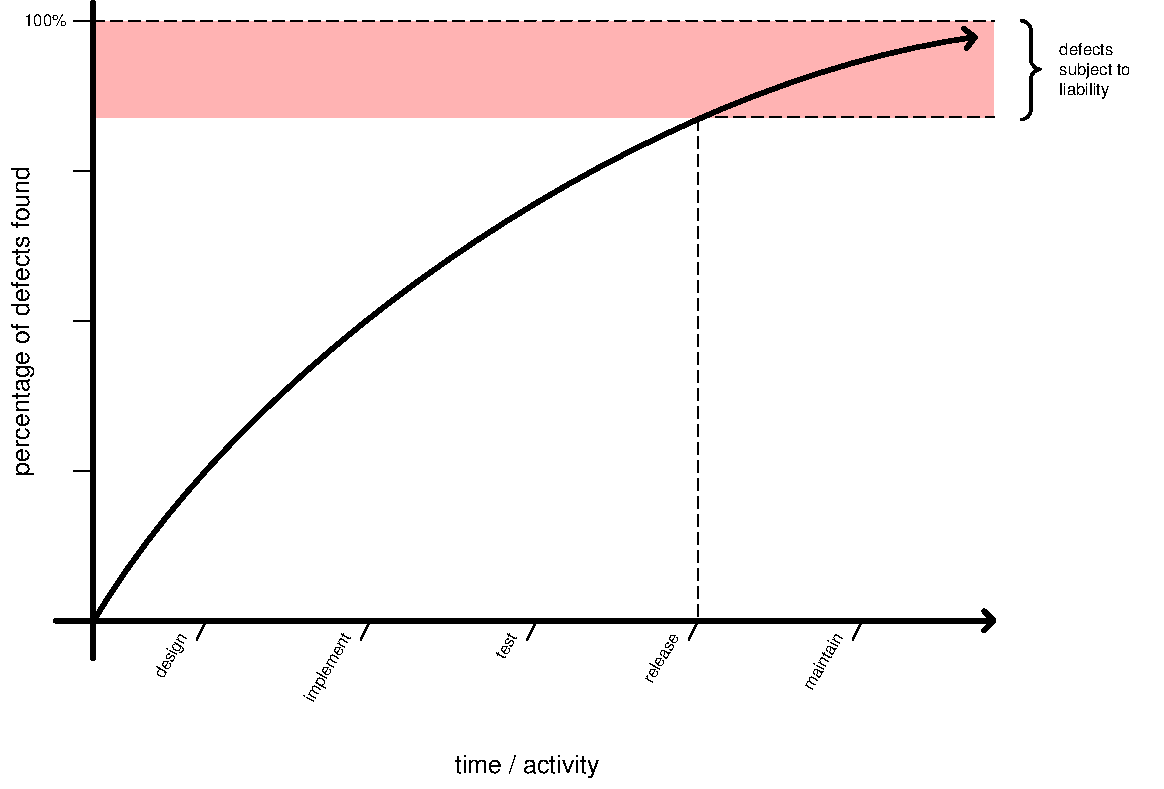
\includegraphics[scale=0.77]{figures/graph.pdf} 
\end{center} 
\caption{Defect Tracking Over Time} 
\label{fig:bugs} 
\end{figure} 

The graph in Figure \ref{fig:bugs} qualitatively illustrates the discovery of engineering defects over time. The y-axis represents the percentage of defects found in a software product. The x-axis represents time starting at the point where engineering begins. Logically, the percentage of defects found increases over time through various engineering best practices. Additionally, as defects are found and fixed, the rate at which they are discovered should theoretically decrease. As time progresses, the percentage of defects found approaches, though very likely never reaches, 100\%. The point in time that the product is released to the public intersects with the defect curve leaving some amount of defects undiscovered. The percentage of undiscovered defects that remain in product \textit{after} it is released is subject to liability. By identifying the best practices that should take place before this point in time, engineers can increase the defects found and repaired before they release to market, thus minimizing the defects subject to liability.

Engineers releasing safety-critical products would love to be able to guarantee 100\% safety, but unfortunately there is no tool to use or process to follow that would allow them to do so \cite{Brooks87}. The edge cases that can cause injury will happen and software engineers will learn from these mistakes. This work is interested in laying out the processes that would at least minimize the risk of safety-critical software and reduce the harm that would result from those defects that are overlooked. To do so, it would be helpful to understand the types defects that software engineers would be held liable to.

\section{On defect classification}
It is necessary to distinguish the type of legal defect a product is held against so that the courts can determine the standard of liability to be imposed--e.g. strict liability or negligence--and thus, the proof necessary to warrant a case. Product defects fall into three categories \cite{Rest3d}: (a) manufacturing defects; (b) design defects; and (c) warning defects. Warning defects are not necessarily part of the actual product and thus this research dismisses this third class of defect\footnote{Turner points out that the duty to warn may not even be applicable to software engineers \cite{Turner99}. If software engineers knew of the specific risks they would be required to warn users about, they should redesign the software to account for them in the first place!}. Manufacturing and design defects are explained more fully below.
\begin{itemize}
\item\textbf{Manufacturing Defect:} Does not conform to specifications.
\item\textbf{Design Defects:} The design itself is unreasonably safe.
\end{itemize}
Research has concluded that software code can easily contain both classes of defect and that the current, practical body of evidence available in software engineering (specifications, documentation, source code) is insufficient for determining the class of defect in arbitrary cases \cite{Turner99}.

Hence, this research seeks to prepare software engineers by discussing the process that can improve defect prevention in both cases. In so doing, this thesis aims to refine the behavior of software engineers in the safety-critical realm to improve the overall safety of their products and avoid the risk of legal dispute.

\section{Summary}

\chapter{Legal Background} 

\begin{quote}
``\textit{\ldots [the law], by the very necessity of its nature, is continually transmuting those moral standards into external or objective ones\ldots}''
\flushright{\textsc{-Oliver Wendell Holmes} \cite{Holmes23}}
\end{quote}

Whether software engineers are aware of it or not, the programs they write are heavily regulated by the law. In software as with many other industries, there is a struggle between safety, cost, and utility. This chapter examines how legal regulation for product safety affects technical design and ultimately the implementation of these products.

\section{Legal Procedure} 

The broad intent of the law is to achieve and preserve justice. In order to assure the safety of products, the law will likely rely on common law principles during disputes. The \textit{common law} regulates based on precedence from judgments found in previous courtroom decisions rather than exclusively on statutes adopted by legislative bodies. 

In the context of safety-critical software engineering, in order for the legal system to be invoked, some sort of disputable accident causing injury must occur. Victims who have suffered loss file a claim. Facts are gathered by searching through evidence and recording testimonies. After all parties agree on the facts, a trial takes place and both sides make arguments calling into question the legality of what occurred using precedent set from previous judgments stored in legal archives. A judge interprets what the law states and either he or a jury decides how it will apply in each individual case. Once the judge renders a decision, cases like this oftentimes undergo an appeal wherein the unsatisfied party petitions a higher court to review the decisions of the lower court to correct potential errors. The parties make more arguments on the legality of the previous decision, but new facts, testimony, and evidence are not accepted. When an appellate decision is made, that holding enters legal archives and serves as precedent for future cases. This process is referred to as the common law. 

\begin{figure}[t] 
\begin{center} 
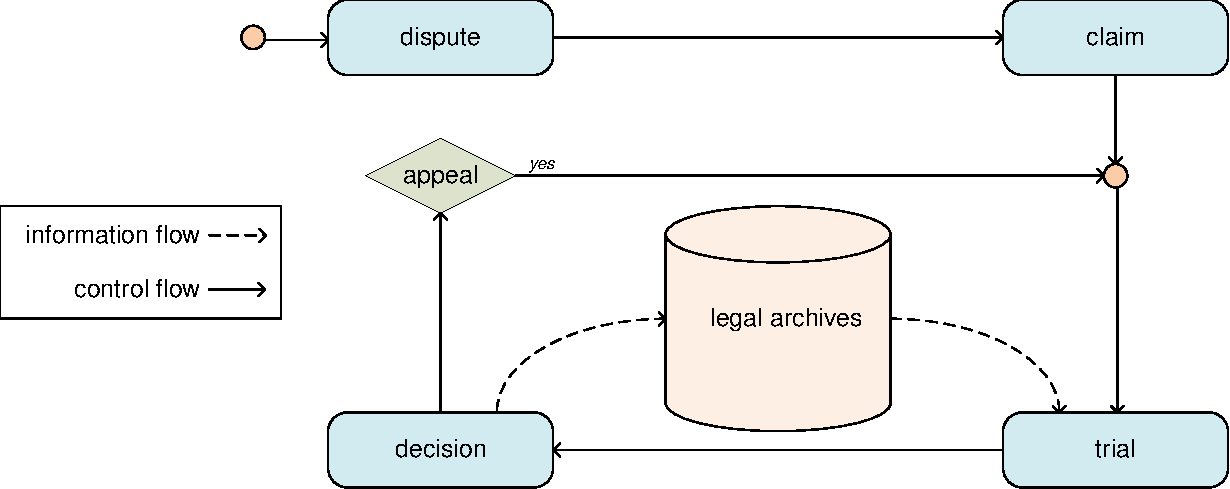
\includegraphics[scale=0.73]{figures/commonlaw.pdf} 
\end{center} 
\caption{Common Law Process} 
\label{fig:commonlaw} 
\end{figure} 

The model in Figure \ref{fig:commonlaw} is a simplification of how the common law system in the United States handles disputes, specifically disputes involving defective products, and updates itself through an iterative feedback process. Input data to the trial includes facts, testimony, and the legal archives which consist of rulings and opinions from previous disputes. These rulings can be used to make decisions in current and future cases and is how the common law updates itself. If an unprecedented situation comes to suit, then the courts interpret similar situations and apply at the discretion of the judge. When a decision is rendered here, it becomes a resource for future disputes.

The particulars of the adjudication process are less important than the core of how the common law functions. What is noteworthy of the model in Figure \ref{fig:commonlaw} is the application of legal decisions to each scenario. Rather than creating statutes from theory, common law cases use actual incident to make decisions about disputes. This means that the litigators, witnesses, and the parties involved in the dispute are, in part, responsible for setting precedent for future cases. Incidentally, this means that the common law is a reactive system because only after accident or injury occurs will legal repercussions be dealt with. When a judgment is made, it can then be applied to future scenarios, but usually only if a lawsuit is filed first. This timeless nature of the common law means that while it is not as easy to interpret as hard statutes, it is, in essence, future proof.

\section{Characteristics of the Common Law} 

The common law is ``that part of the law that is within the province of the courts themselves to establish'' \cite{FAKE}. It exhibits many characteristics that make it just. Social propositions (those of morality, policy, or experience rather than state legal rules) are enforced impartially to any party. The courts practice a replicable system of litigation, allowing future disputants to receive legal advice. The common law is also responsive to change as moral norms evolve over time \cite{FAKE}. 

Those who are affected by the common law should understand the basic principles of its underpinnings. Software engineers working on safety-critical projects are pressured by social expectations for reliable and functional software. But because of its unique nature, defects in software are inevitable and typically more difficult to locate and fix than the physical flaws found in mechanical components \cite{Parnas90}. Defects in software used in safety-critical situations can be especially dangerous. The increasing use of software in machines and the demand for more products functions adds additional complexity and room for error.

Fortunately, the legal system can account for this inherent complexity. For disputes resulting in injury or death from defective software, the most appropriate claim a plaintiff can make against software engineers will be of tortious behavior of the defendant. A \textit{tort} is a civil (not criminal) wrong or breach of duty to another person. Courts chosen to resolve these types of disputes will tend towards regulation through products liability law \cite{FAKE}. Products liability is almost exclusively regulated by common law decisions, meaning that cases under it must be resolved by applying rules generated by prior decisions. In addition to being applicable to software related disputes, products liability law resolves some of the complexity found in safety-critical software because disputes are closely examined on a case-by-case basis and there are no strict universal statutes that would simplify a decision.

\section{Products Liability} 
The term \textit{products liability} is the area in law that broadly applies to the liability of a manufacturer or seller for injury to a buyer caused by a product that they sold \cite{FAKE}. A \textit{product} usually refers to physical merchandise that can be purchased. Officially, a product is defined as 

\begin{quote}
``\textit{\ldots tangible personal property distributed commercially for use or consumption and other items, such as real estate property and electricity, when the context of their distribution and use is sufficiently analogous to the distribution and use of tangible personal property\ldots} (\cite{Rest3d}, \S19(a))'' 
\end{quote}

In the case of safety-critical systems, software is usually embedded in some machine or hardware device \cite{Leveson95} that is sold as a product. When viewed from this standpoint, software is less analogous to pure thoughts and expressions and is considered a product for products liability cases. Regardless, this research assumes that software is considered a product.

Within products liability, a tortious act can be classified as either strictly liable or negligent \cite{Turner99}. Strict liability applies to any product that is defective, regardless of the process used to manufacture. While strict liability is interesting, this research is concerned with the \textit{process} used to build software and how engineers employ it. Since process is behavioral, it falls under the jurisdiction of negligence.

\subsection{Negligence}

Negligence is more concerned with the process used to build a product, not the product itself. Because manufacturing or design based defects are difficult, in fact nearly impossible, to classify \cite{Turner99}, applying negligence to software related incidents is even more appropriate. In general, the legal term \textit{negligence} refers to careless conduct. Scholars describe negligence\footnote{\textit{See:} 57A Am. Jur. 2d Negligence \S 5} more specifically as:\singlespace
\begin{itemize}
 \item the existence and violation of a legal duty to use care, proximately 
 causing injury to another.
 \item the failure to exercise the degree of care demanded by the circumstances.
 \item the breach of a duty to another to protect him or her from the particular
 harm that ensued.
 \item the want of that care the law prescribes under the particular
 circumstances existing at the time of the act or omission which is involved.
\end{itemize}\doublespace
Negligence can be applied to many different scenarios beyond products liability. An intoxicated driver who disobeys traffic laws may be negligent towards other citizens of the road\footnote{\textit{See: People v. Townsend}, 214 Mich. 267, 272, 183 N.W. 177.}. A instructor who fails to demonstrate safety precautions to his students in wood shop may be liable for negligence\footnote{\textit{See: Voorhies v. Conroe Independent School Dist.}, 610 F.Supp. 868.}. An engineer who does not adequately inspect his safety-critical product can be negligent to his clients\footnote{\textit{See: Ford Motor Co. v. Mondragon}, 271 F.2d 342.}. This research focuses on the negligence constrains as they apply to products liability.

Negligence is easiest to determine when some standard of care stated by the profession is available. Lawyers are held to a standard defined by their state's Bar Association and doctors are licensed by the state's medical board. But while there are standards and best practices defined for software engineers \cite{FAKE}, no similarly legal official standard exists for software engineering. A more qualitative approach must be taken. The duty of software engineers are expected to fulfill is that of one who is reasonably prudent. Reasonably prudent software engineers would use the best available technologies at a reasonable cost and follow what is, at the time of implementation, considered to be the industry ``state-of-the-art''.

Figure \ref{fig:handtest} shows a formula that equates negligence in terms of unreasonable behavior.  According to the Learned Hand test\footnote{\textit{See: United States v. Carroll Towing Co.}, 159 F.2d 169.\\ Judge Learned Hand created this guideline to determine the amount of duty owed in a negligence dispute. In the case, the United States sought compensation for flour that was lost when a barge carrying the cargo sunk. The barge company was partly responsible because no workers were present on the barge when it sank, which may have prevented the barge from sinking. Qualitatively, the amount it would have cost to keep a worker on the barge would have been less than the product of the probability that the barge sank and the amount of damages incurred from it sinking.}, an organization that develops safety-critical software has a duty to spend at least the amount of time and resources equivalent to the product of the severity of harm and the likelihood that it will happen. If they do not, then their actions are negligent. The Learned Hand test is an important metric because it provides a way to evaluate the existence of negligence without the presence of a strict standard.

\begin{figure}
\begin{narrow}{-1.5in}{-1.5in}\begin{center}
\begin{tabular}{|l|}
\hline
	Let \textbf{B} be the burden (expense) of preventing a potential accident.\\
	Let \textbf{L} be the severity of the loss if the accident occurs.\\
	Let \textbf{P} be the probability of the accident.\\[6pt]
	Then \textit{failure to attempt to prevent a potential accident is 
	unreasonable if}\\[8pt]

      \centerline{\(B < P \times L\)}
\\[3pt]
\hline
\end{tabular}
\end{center}\end{narrow}
\caption{The Learned Hand Test for Negligence}
\label{fig:handtest}
\end{figure}
\subsubsection{Elements of Negligence}
The laws of negligence can only be invoked under certain conditions. The prerequisites, or prima facie elements, of a negligence case are that \cite{Dobbs01}:
\singlespace
\begin{enumerate}
 \item there exists a duty of care (or duty to protect)
 \item the defendant breaches this duty with unreasonably risky conduct
 \item the defendant's conduct resulted in harm to the plaintiff
 \item the negligent conduct was a proximate cause of harm
 \item legally recognized damages or injury exist
\end{enumerate}
\doublespace
In \textit{The Case of the Killer Robot}\footnote{\textit{The Case of the Killer Robot} is a fictional scenario created by Richard G. Epstein to illustrate the complexity of building real-world software and the ethical issues introduced in the safety-critical realm. It is referenced in \cite{Epstein96} and reprinted with academic permission in Appendix \ref{appa}.}, employees of Silicon Techtronics Inc. wrote software for robotics that were to manufacture products at Cybernetics Inc. The software contained latent defects that ultimately lead to the death of Cibernetics employee Bart Matthews. This fictional scenario poses an ideal case study for the legal issues surrounding software development and the applicability of negligence.

Negligence cases call for an actual duty of care owed to a plaintiff. There may be a question about how much care is owed in a given situation, but there are circumstances in which there is no duty owed that bears on the harm a plaintiff suffers. Judges decide whether or not this duty exists. In the killer robot example, Silicon Techtronics Inc. is held to a duty of care expected by users of their machinery. Since their software controls machines that are capable of injuring humans, it is reasonable for users to expect some amount of care to be taken to prevent this.

Also, there must be a breach of this duty of care owed. A defendant who behaves reasonably and exercises the necessary care required by law will not be negligent even if the plaintiff is harmed. The facts in the killer robot case evidence that Silicon Techtronics breached this duty. Their development practices were questionable at best, but factors like utility and practicality should be brought into question.

The defendant's negligence must be the cause of the harm suffered by the plaintiff. A careless engineer who does not test his product is not negligent to the user who is injured by tripping over the machine. In addition, the cost must not only be the cause in fact, but a proximate, or primary cause of the harm suffered. This requirement is difficult to apply in the killer robot case. While it can be argued that Silicon Techtronics' processes did not follow the software engineering state-of-the-art, it is difficult to prove that this allegedly negligent behavior actually lead to the mistakes that Randy Samuels made.

Finally, actual damages or injures must be suffered for a negligence case to follow suit. This can include personal injury or damages to property.

\subsubsection{Why hasn't our legal system addressed software negligence?} 

The American legal system has still yet to resolve a \textit{real} dispute involving software. As software has now been around for decades and has already caused problems worthy of litigation \cite{FAKE}, why havent our courts regulated for safer software? 

One reason why our courts have not addressed the issue of software safety is because of out-of-court measures that companies will take to settle disputes. Oftentimes, disputes will be settled through mediation, wherein a neutral third party facilitates a compromise of the situation \cite{FAKE}. Unfortunately, the law does not get updated through mediation because this kind of dispute resolution does not make a determination of right or wrong, it merely creates an agreement not to pursue trial litigation. Authority that constrains trial court judges, and subsequently software engineers that face such trials, is only developed by appeals courts. Appellate review produces the legal requirements and constraints for real trials. 

Often, cases will be dismissed in real trials because of out-of-court settlements wherein the defendant compensates the plaintiff at an amount agreed upon by both parties.

\section{Addressing Cost}

While the legal system (among other things) ensures the safety of products, the law understands the costs involved in ensuring safety measures and takes this into account when resolving disputes. Scholars posit that the law balances these economic forces and ensures safety to a reasonable cost to manufacturers \cite{FAKE}.

Some lawyers contend that the law evolves towards efficient decisions in accident disputes in courts, where ``\textit{efficient}'' in this context means the defendant-manufacturer is more likely than the plaintiff-victim to win the suit if an accident occurs. In terms of software engineering, this means that an organization that develops safety-critical software will, in the long run, tend towards winning or possibly avoiding dispute. This is a good thing because it means the quality and safety of software improves. In fact, software quality and safety must improve if the defendants are to win, and possibly avoid, dispute. The party that is interested in precedent (in this case, the defendant software developers) will litigate until a favorable decision is met. This means that manufactures that are likely to be involved in accident disputes will make preventative efforts to improve the safety of their products to avoid liability costs in court cases and more easily defend themselves in case of a dispute \cite{FAKE}.

\section{Summary}

\chapter{Software Processes} 
In order to build quality software systems, many organizations follow a formal approach to the software development process including formal methods, best practices, and adoption of standards. One such methodology, the Spiral Model of Software Development and Enhancement, has withstood the test of time and is still widely accepted as the state-of-the-art in software process. Diligent adoption of this model, be it intentional or incidental, can in many ways fulfill the ``due care'' requirements set forth by judicial authorities. 

\section{Basic Models of the Software Process} 
The following concepts are not explained in depth, as it is assumed that the audience of this section is already familiar with these basic ideas of software development. Later sections explain how prudent application of these practices fulfills the legal requirements set forth by the common law. 

\textbf{Design}: Herb Simon would classify design in general as the formulation actions that will ``change existing situations into preferred ones''. From software engineering standpoint, designers are concerned with how things ought to be in order to attain goals and function \cite{simon}. Activities can include gathering requirements, developing external functions and interfaces, designing internal component structures, generating test plans, and ensuring functions are complete and achievable. 

\textbf{Implement}: The implementation phase of the software cycle involves the translation of design into functional code. Sometimes referred to as software construction or coding, engineers will implement code to create a static description of the processes defined in the prior phase, usually in the form of a programming language. 

\textbf{Test}: Testing is the validation of the implementation against the programs design. This can be done through a variety of ways including, but not limited to, unit and system testing, black box testing, static code analysis, and automated testing. Testers seek to discover defects so that engineers can fix them before the code is released to the public. 

\section{Reasonably Prudent Software Development} 
discuss software development practices that satisfy legal constraints. discuss methodologies (waterfall, spiral) that help improve quality of software. discuss the academic field and what they teach in universities. bring up the code of ethics.  

then discuss actual, formal standards set forth by the ieee, acm, etc. bring up those ieee standards you find and show how they meet legal standards.  

software engineering must be proactive to prevent bugs from getting released, while the common law is reactive. 

While certain design defects can occur during the design phase, these flaws will still manifest themselves as errors in the actual source code. It is agreeable that certain design activities related to requirements occur \textit{during} development \cite{Turner99}; that is after software construction has started. Because the source code is where flaws will ultimately need to be fixed, this work is interested in those activities that can help prevent software defects that would manifest after construction has begun.

\textbf{Design}: Defects in design are difficult to prevent as there are no automated tools to detect them. By analyzing risk and borrowing the best practices from the state-of-the-art, software designers can reduce the number of defects that get written into the code.

The state-of-the-art in design is extensive. Design involves analyzing requirements and writing specifications.

\textbf{Implement}: Implementation involves converting the specifications from the design into actual software code. Reasonably prudent software engineers use modern tools and distinct methodologies to implement software.

The state-of-the-art of software implementation is constantly evolving. Software compilers translate human-readable code written by programmers into machine bits or byte/object code. Syntax mistakes and simple error conditions can be detected by compilers and prevent software defects. Compilation typically happens soon or immediately after a programmer finishes a unit of programming work. But advanced integrated development environments often provide real-time compilation that happens during development so that these simple errors are detected as the programmer is writing code. 

As software has matured, certain programming practices have been universally recognized as the state-of-the art. Static code analyzers like FxCop or FindBugs are more sophisticated than a compiler and can detect certain violations of these best-practices. Analyzers can detect potential dynamic, or runtime errors, without actually executing the code. This is beneficial because reproducing every possible code path in tests is difficult, and arguably impossible, to achieve. Static code analysis typically happens after a complete unit of programming finishes and an analyzer can run on either the source or object code.

There are also several implementation methodologies that can be considered state-of-the-art depending on their application. Pair programming and extreme programming are examples.

\textbf{Test}: When software is complete enough to be executed, a series of unit and system level tests run to validate the code against its expected behavior. In  addition to automated test cases, test engineers run black-box style tests to mimic real-world usage. 

\section{Summary}

\chapter{Paving the Intersection} 
we don't have to wait and be reactive like the common law. we have influence right now! it may not seem like it, but software engineers can indirectly influence law in the following ways: 
academics and research (expert testimony) 
standards and committees (ieee, acm, etc.) 

\section{Scopes of Influence} 

In a legal context, different perspectives are used to scrutinize the liability of software. Each perspective has its own scope to which it can influence its encapsulated perspectives. The initial level is the software implementation perspective. To determine liability based on a manufacturing defect, the implementation is scrutinized against the engineers' design of the product. Thus, the implementation perspective is encapsulated by the design perspective. 

Beyond a simple manufacturing defect liability, software engineers can also be negligent if their design is unsafe. To determine negligence, the design itself is judged against a standard outside of the specification of the project. Courts normally refer to this outside standard as the ``State-of-the-Art. This perspective is used to determine if the behavior of software engineers, in the form of their design, was negligent. The state-of-the-art can influence a software products design, and by virtue its implementation, because its perspective has a wider scope than software design. 

While software engineers are in fact held accountable by a legal system that, by itself, lacks the technical merit to pass judgment on such a specialized field, they can influence the very standard against which they are judged. Software engineering experts from both industry and academia, by the very nature of their work, define what constitutes the state-of-the-art. Thus, two more perspectives are introduced whose scopes encapsulate all others: Academia and Industry. Both perspectives have, qualitatively, equal influence over the software engineering state-of-the-art and its underlying perspectives so one cannot encapsulate the other. However, since both perspectives borrow expertise from one another, they can mutually influence each other. 

\section{Summary}

\chapter{Conclusion} 
Software safety, for now, remains an impracticable desire. While the precautions and recommendations derived from this research can assist in improving the overall safety and quality of software products, they cannot be held to the same regard as professional standards. The software industry still needs time to mature and society must learn to recognize that software is engineering. 

\section{Drawbacks and Limitations} 
Building software with safety constraints affirmed to the same level as medicine, architecture, or even other fields of physical engineering, is unlikely to happen within the near future. Certain inequities of the industry and limitations of the medium prevent software engineers from ensuring the safety of software like other industries are able to. 
Just as the software profession is lacking in legal history, these legal shortcomings mutually hinder the effectiveness of software engineers. 

\subsection{Why We Can't Guarantee Software Safety} 
Society is accustomed to software solutions built faster and cheaper. Imposing constraints to improve safety will slow down the speed in which developers can implement solutions; a speed at which safety-critical clients already expect them to deliver at. In addition, adding longer and more thorough development patterns will add to the cost of the solution. But if the cost of a safer software solution is slower and more expensive to build, clients may not see any value of using software over traditionally engineered solutions.

Software development jobs are not all safety-critical. Unlike other professions, the vast majority of jobs available to computer science graduates are in enterprise and end-user software that is not safety-critical [cite:? monster]. Since these areas do not need safety-regulation the way that all doctors, architects, and physical engineers do, progress in software safety is obstructed. 

\subsection{Why We Shouldn't Guarantee Software Safety} 
Creating a strict standard will hinder technical progress. Software is still in a state where it is evolving quickly, and if a hasty standard is created, it will either halt technical progress at the point where the standard is, or will quickly become obsolete and unable to catch up to the progress that non-safety-critical software developers are working on. 
A defined standard may reduce software quality. Again, since software progress is moving so quickly, software engineers could choose to only follow a standard which at the time is obsolete and insufficient for proper safety. If the safety of an application is evaluated on a case-by-case basis, engineers should take the necessary precautions beyond what is considered sufficient to guarantee safety because there is no minimum to meet. 

\section{Future Work} 

It would not be difficult to expand this research beyond the scope of test. Standards and practices exist for other stages, as well as legal requirements. Much of what has been written can be generalized to other areas of the software development process. 

\bibliographystyle{acm} 
\addcontentsline{toc}{chapter}{Bibliography} 
\bibliography{references} 

\end{document} 
